\item The graph of $f'(x)$ is given below for some function $f$. \newline
(Note:  this is the graph of the \textit{derivative} of $f$) 
\begin{center}
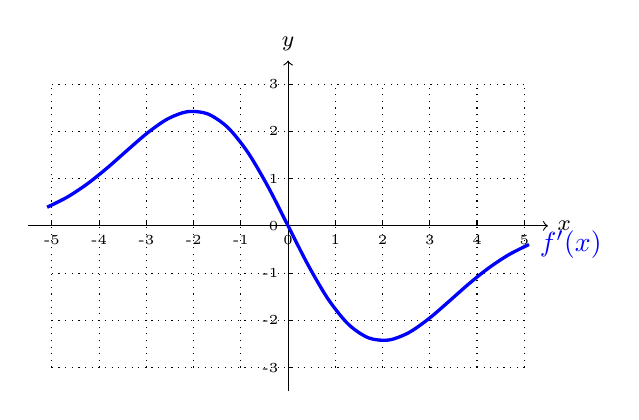
\begin{tikzpicture}[scale=0.6]
\foreach \x in {-5, -4, ..., 5}
{
	\draw[thin, dotted] (\x, -3) -- (\x, 3);
}
\foreach \y in {-3, -2, ..., 3}
{
	\draw[thin, dotted] (-5, \y) -- (5, \y);
}

\foreach \x in {-5, -4, ..., 5}
{
	\draw (\x, 0.1) -- (\x, 0) node[anchor=north]{\tiny \x};
}

\foreach \y in {-3, -2, ..., 3}
{
	\draw (0.1, \y) -- (0, \y) node[anchor=east]{\tiny \y};
}

\draw[->] (-5.5, 0) -- (5.5, 0) node[anchor=west]{\footnotesize$x$};
\draw[->] (0, -3.5) -- (0, 3.5) node[anchor=south]{\footnotesize$y$};

\draw[variable=\x, domain= -5.1:5.1, smooth, very thick, blue] plot ({\x}, {-2*\x*exp(-\x*\x/8)}) node[anchor=west]{$f'(x)$};
\end{tikzpicture}
\end{center}

On which of the following intervals is $f$ decreasing?

\begin{multicols}{2}
\begin{enumerate}\setlength{\itemsep}{.5 cm}
\item $(0, 5)$ %correct
\item $(-5,-2)$
\item $(0, 2 )$
\item $(-2, 2)$
% \item None of the above
\end{enumerate}
\end{multicols}